Auf dem Swipe-Seiten (Abbildungen \ref{fig:swipescreen_alle}) findet die Bewertung der Filme statt. Durch das hier verwendete Matchingsystem mithilfe des Filmgeschmacks unterscheidet sich StreamSwipe von anderen Apps und erhält so einen innovativen, individuellen Charakter, womit diese Seite das Herzstück der App bildet.\\
Das zuvor eingeführte Farbschema bleibt auch hier erhalten, wie Abbildung \ref{fig:swipescreen_a} zeigt. Eine Überschrift im selben Stil wie bereits aus Abschnitt \ref{sec:homescreen} bekannt, verdeutlicht durch eine Frage nach welcher Motivation die Filmauswahl getroffen werden soll. Zentral im Bild ist eine Liste von Postern der zu beurteilenden Filme. Wie bereits durch die Dating-App Tinder verbreitet, werden die Antwortmöglichkeiten durch eine Swipe-Bewegung in eine Richtungen ausgewählt. In diesem Fall werden vier Entscheidungsmöglichkeiten auf vier Richtungen verteilt. Abhängig von der Position des Fingers auf dem Touchscreen bewegt sich das Filmposter innerhalb des Bildschirms, was den Effekt einer frei beweglichen Karte hervorruft. Um klarzustellen welche Swipe-Richtung für welche Entscheidung steht, verfärbt sich der jeweilige Indikator in der unteren Reihe bei Verschiebung des Filmposter. Beide Animationen sind in Abbildung \ref{fig:swipescreen_d} zu sehen. Die Indikatoren sind mit Icons versehen, zeigen aber durch Drücken welche Entscheidung sie repräsentieren und in welche Richtung der Nutzer dafür wischen  muss, wie Abbildung \ref{fig:swipescreen_c} am Beispiel des rechten Indikators zeigt. \\
Durch Antippen des Filmposters werden weitere Informationen zu dem jeweiligen Film dargestellt, wie in Abbildung \ref{fig:swipescreen_b} zu sehen. Gleichfalls wird durch ein einfaches Antippen wieder zurück  zu den Postern gewechselt. Eine Rotations-Animation verdeutlicht die Illusion der Karten.\\
Alle diese für die Bedienung der App grundlegenden Steuerungen verlangen keine feinmotorischen Eingaben und können problemlos von Personen mit motorischen Einschränkungen genutzt werden. Auch dieser Bildschirm ist vollkommen mit Semantiken ausgestattet. Anstelle des Filmposters wird der Name des Films ausgelesen und für die vier Indikatoren am unteren Rand werden jeweils deren Funktion und durch welche Swipe-Richtung sie erreicht werden vorgelesen. Sämtliche Textfelder können ebenfalls problemlos von einem Screenreader gelesen werden.



\begin{figure}[H]
	\begin{subfigure}{0.33\textwidth}
	\centering
	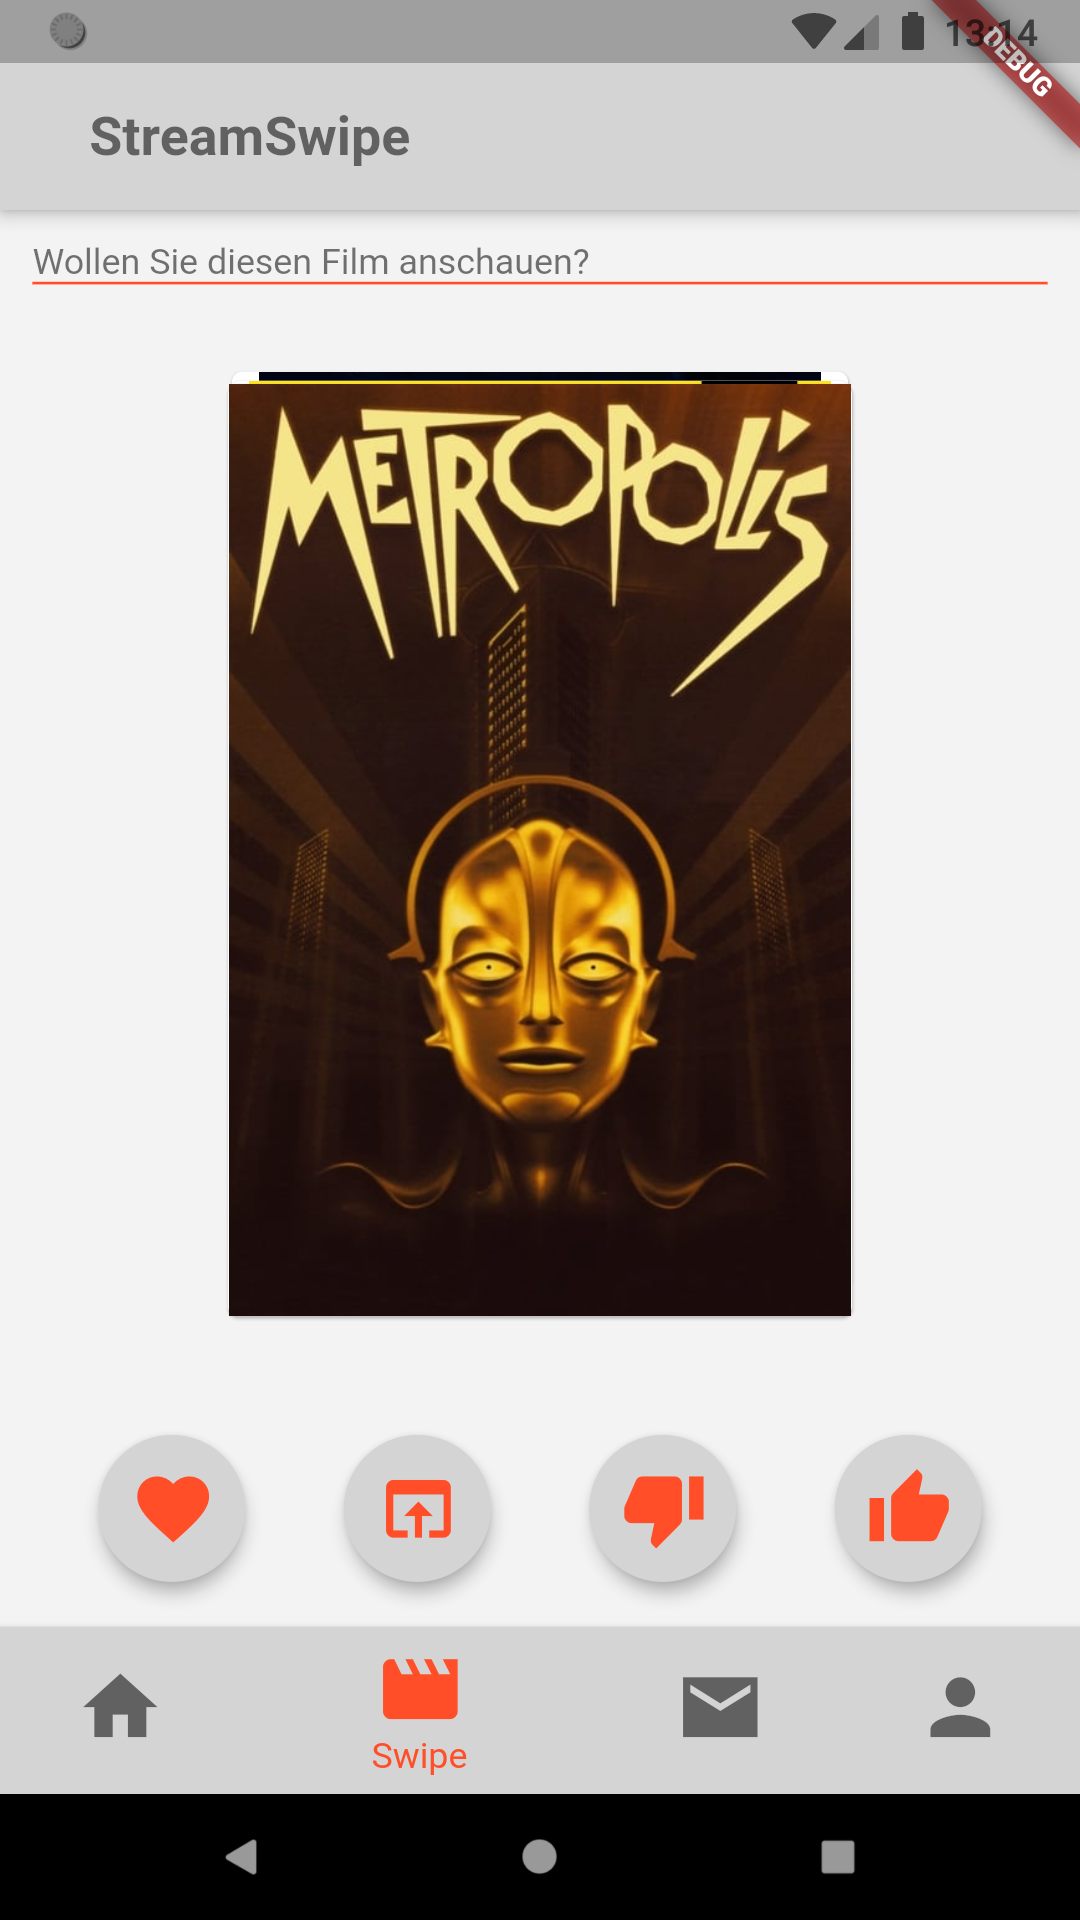
\includegraphics[scale=0.13]{Benutzeroberfläche/images/screenshot_swipescreen1.png}
	\caption{}
	\label{fig:swipescreen_a}
	\end{subfigure}
	\begin{subfigure}{0.33\textwidth}
	\centering
	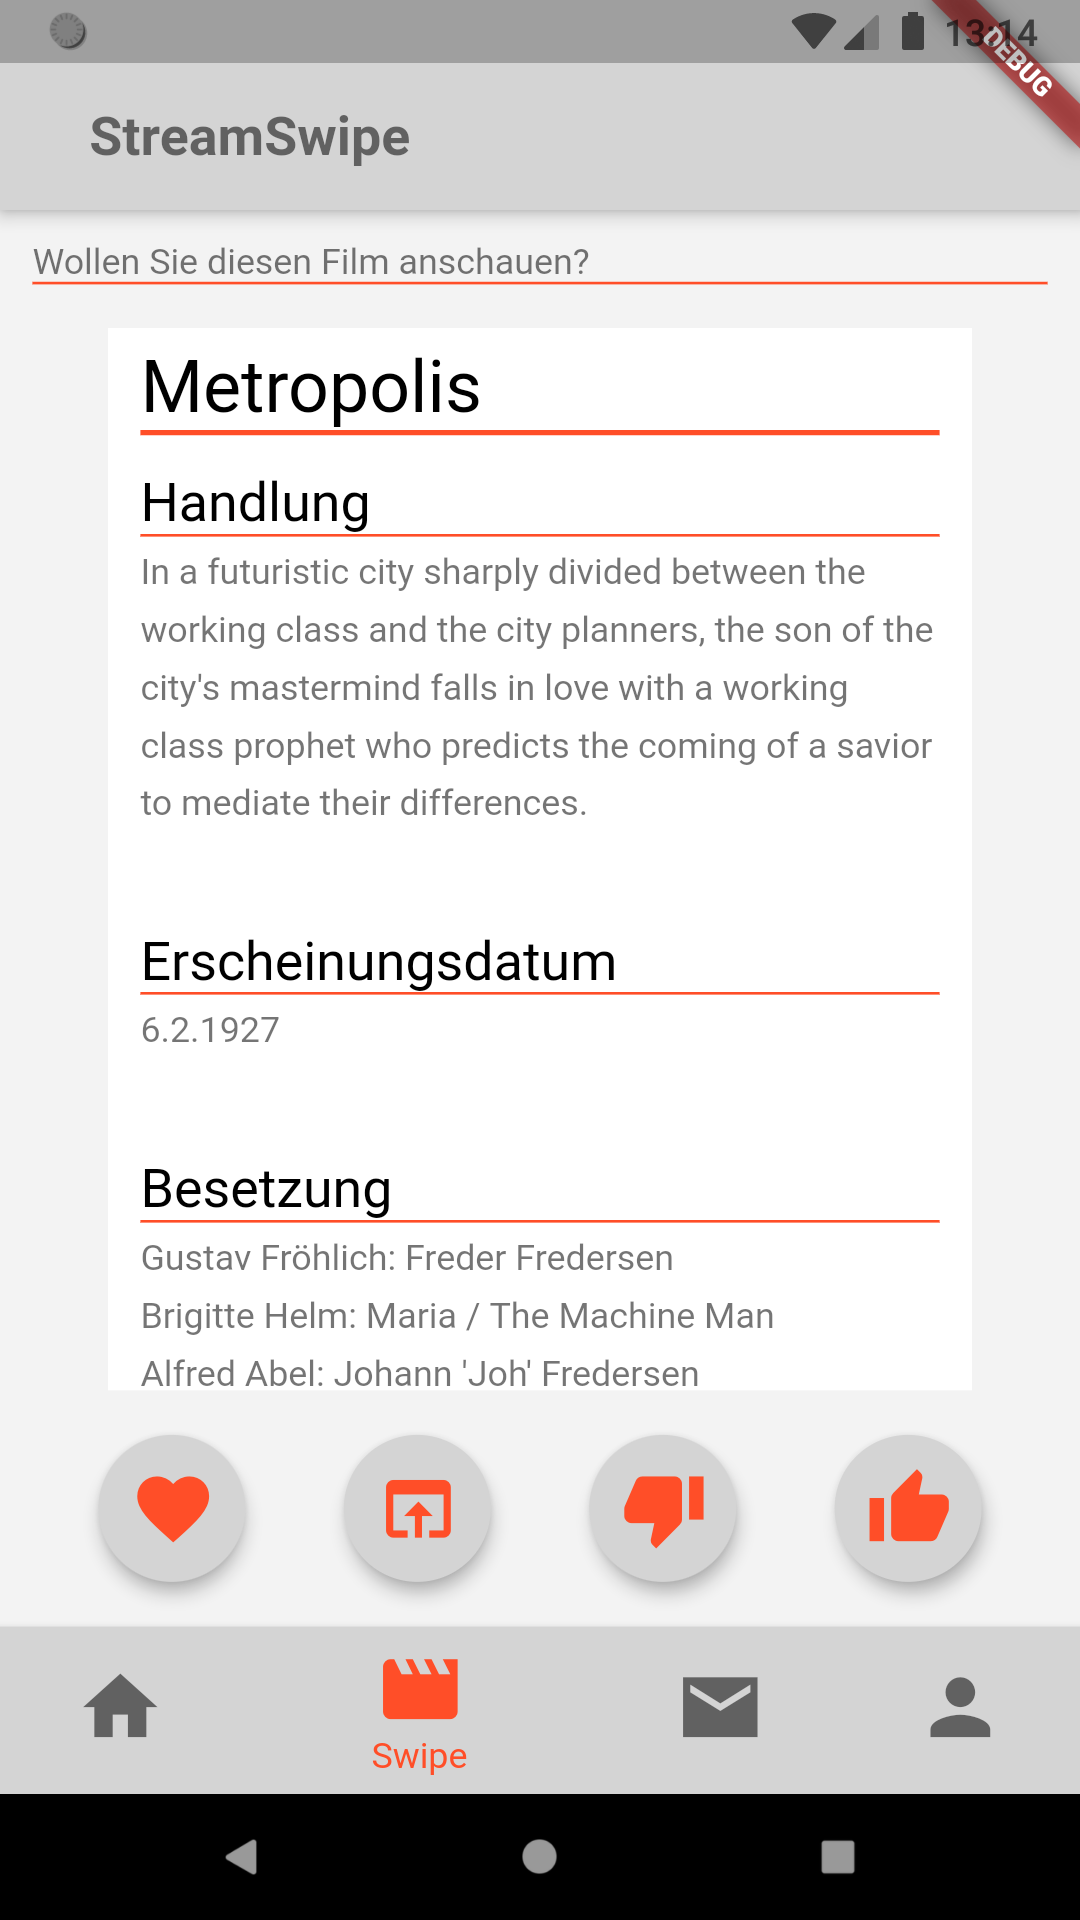
\includegraphics[scale=0.13]{Benutzeroberfläche/images/screenshot_swipescreen2.png}
	\caption{}
	\label{fig:swipescreen_b}
	\end{subfigure}
	\begin{subfigure}{0.33\textwidth}
	\centering
	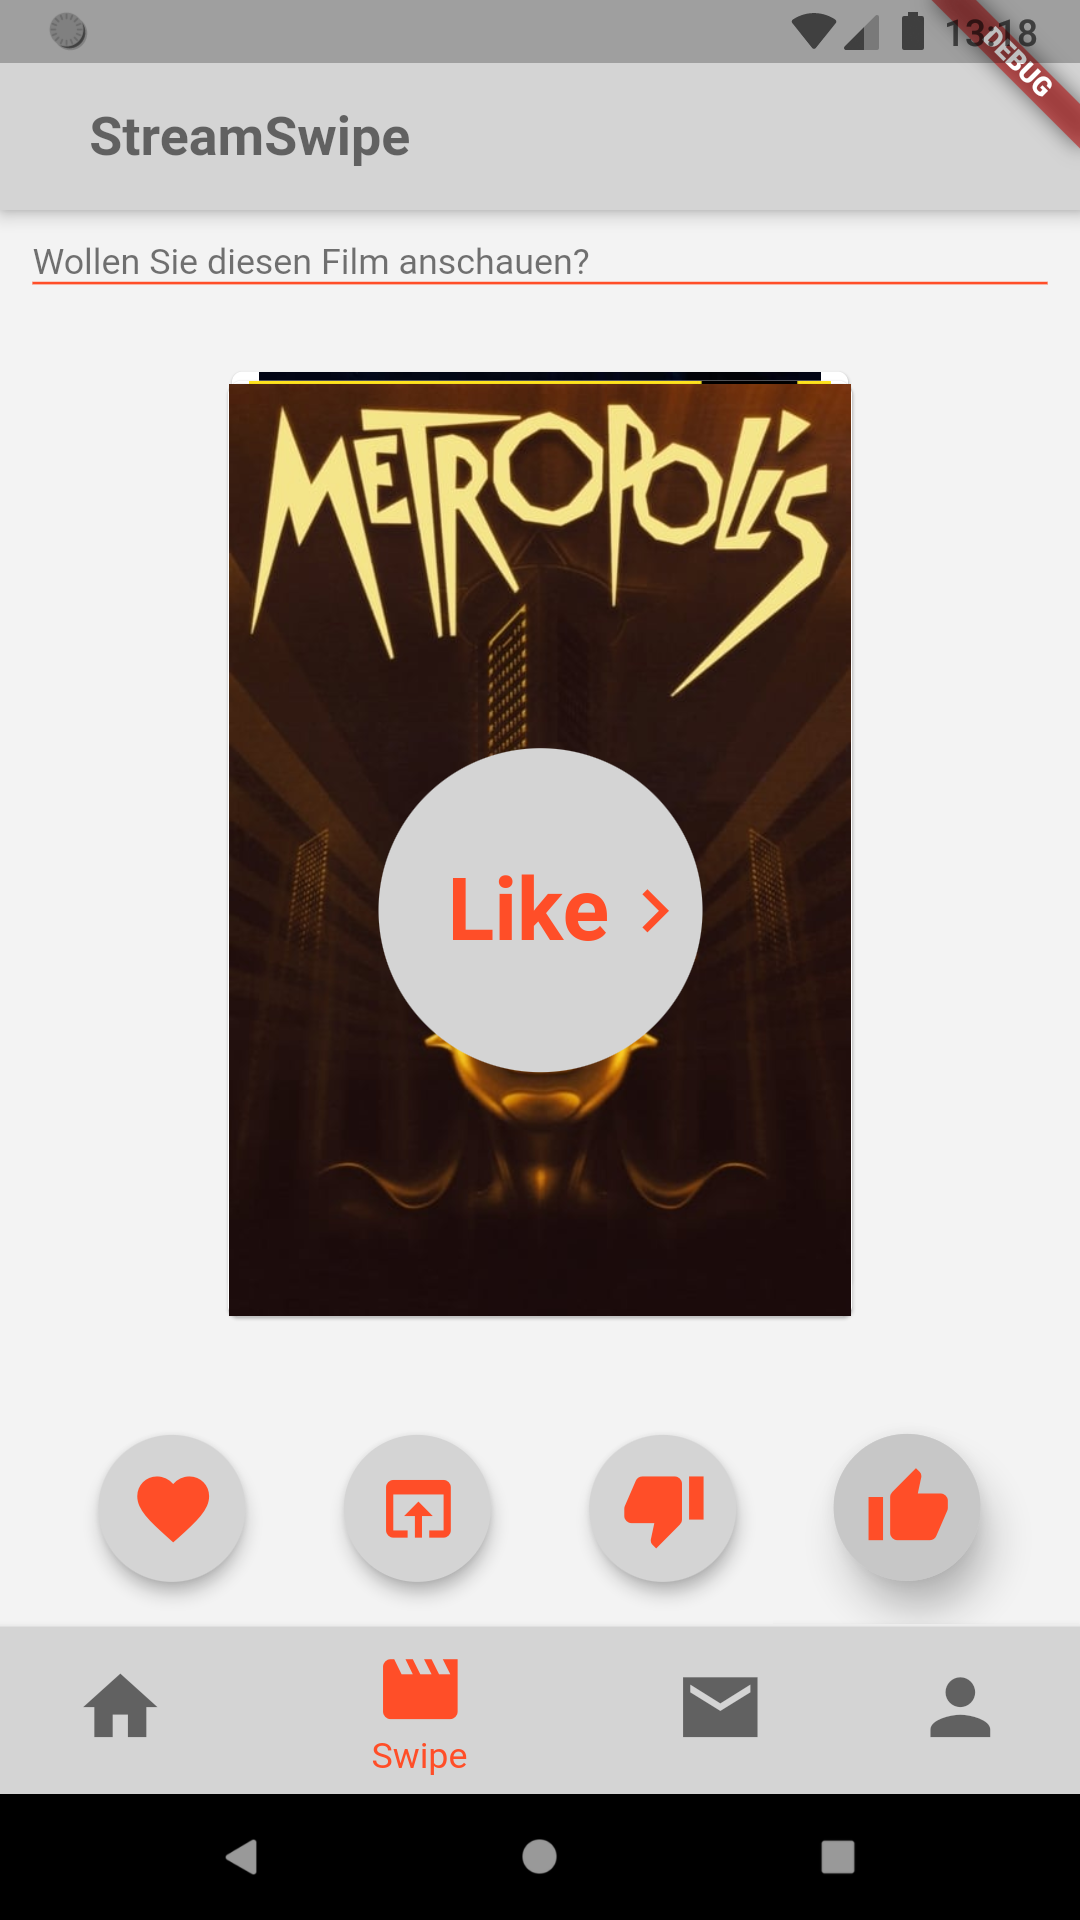
\includegraphics[scale=0.1742]{Benutzeroberfläche/images/screenshot_swipescreen3.png}
	\caption{}
	\label{fig:swipescreen_c}
	\end{subfigure}\\ \vspace{1cm}	
	
	\begin{subfigure}{0.33\textwidth}
	\centering
	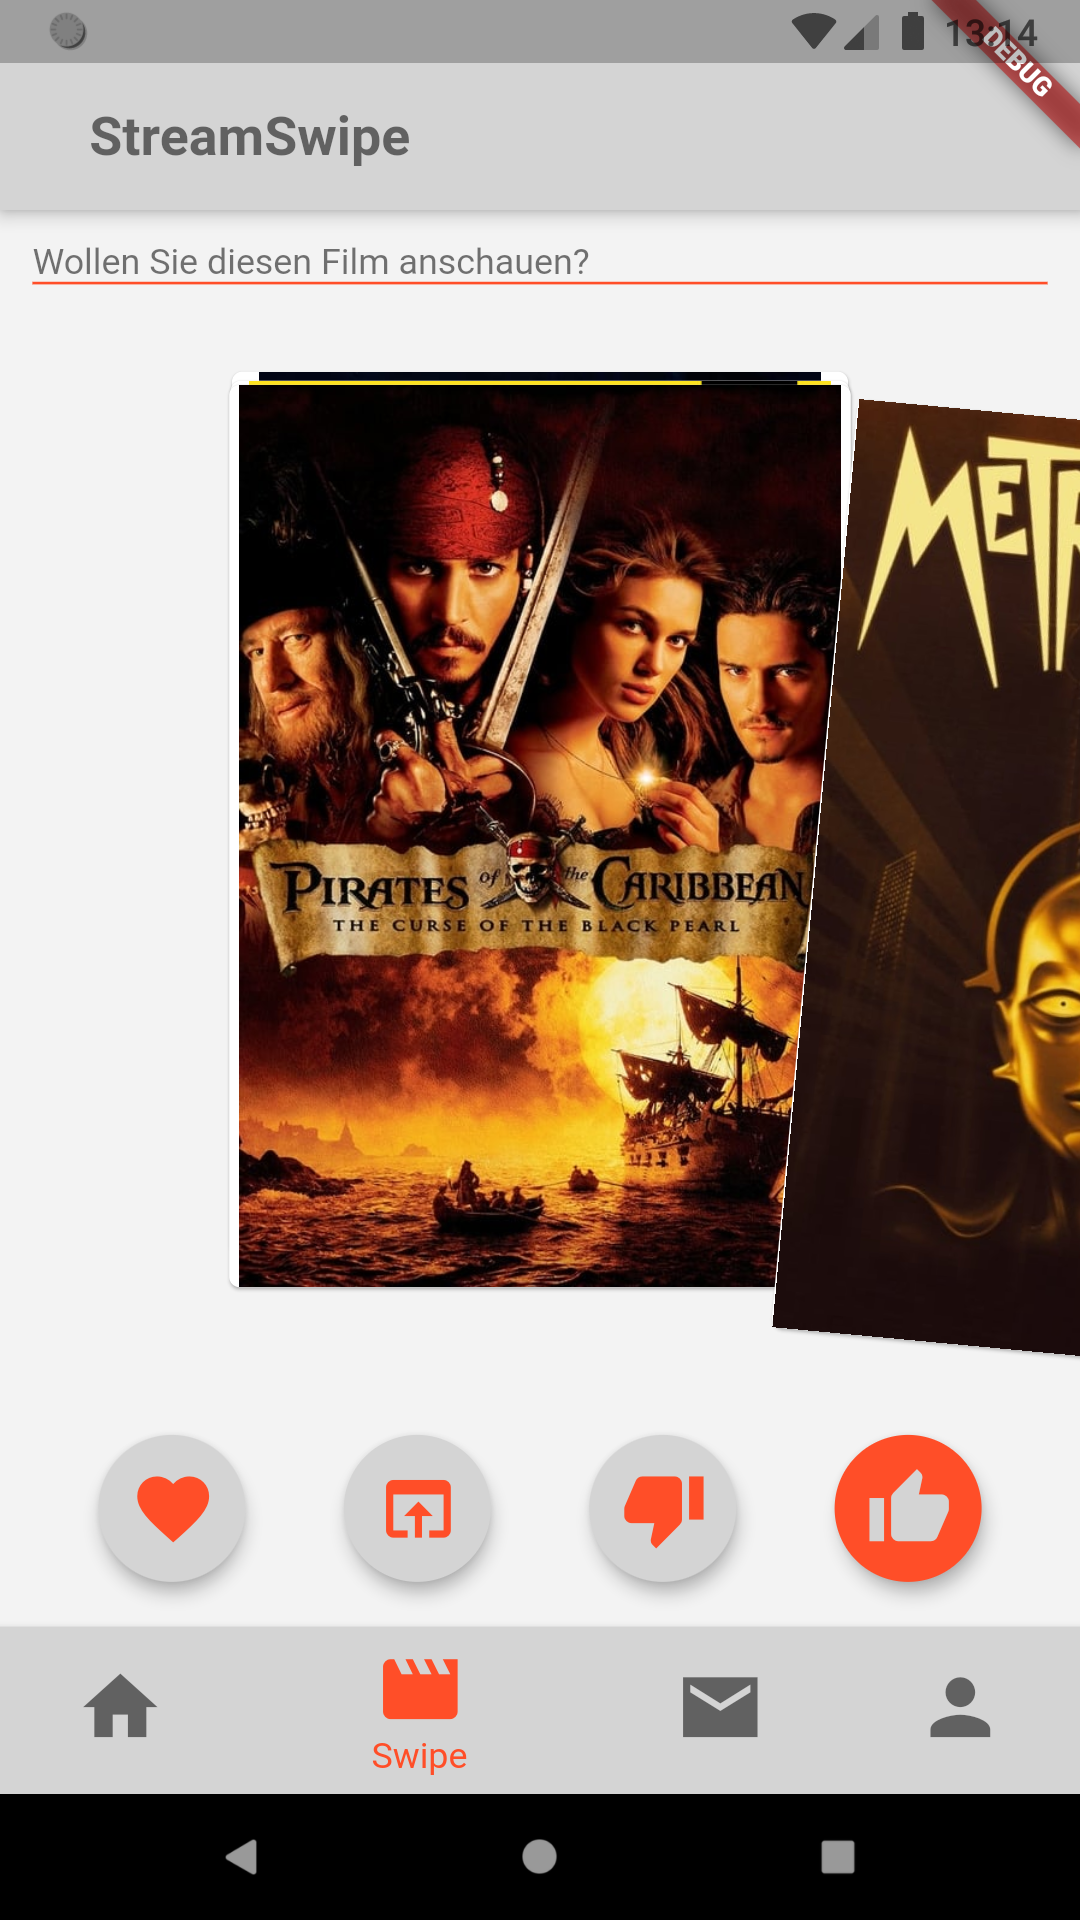
\includegraphics[scale=0.13]{Benutzeroberfläche/images/screenshot_swipescreen4.png}
	\caption{}
	\label{fig:swipescreen_d}
	\end{subfigure}
	\begin{subfigure}{0.33\textwidth}
	\centering
	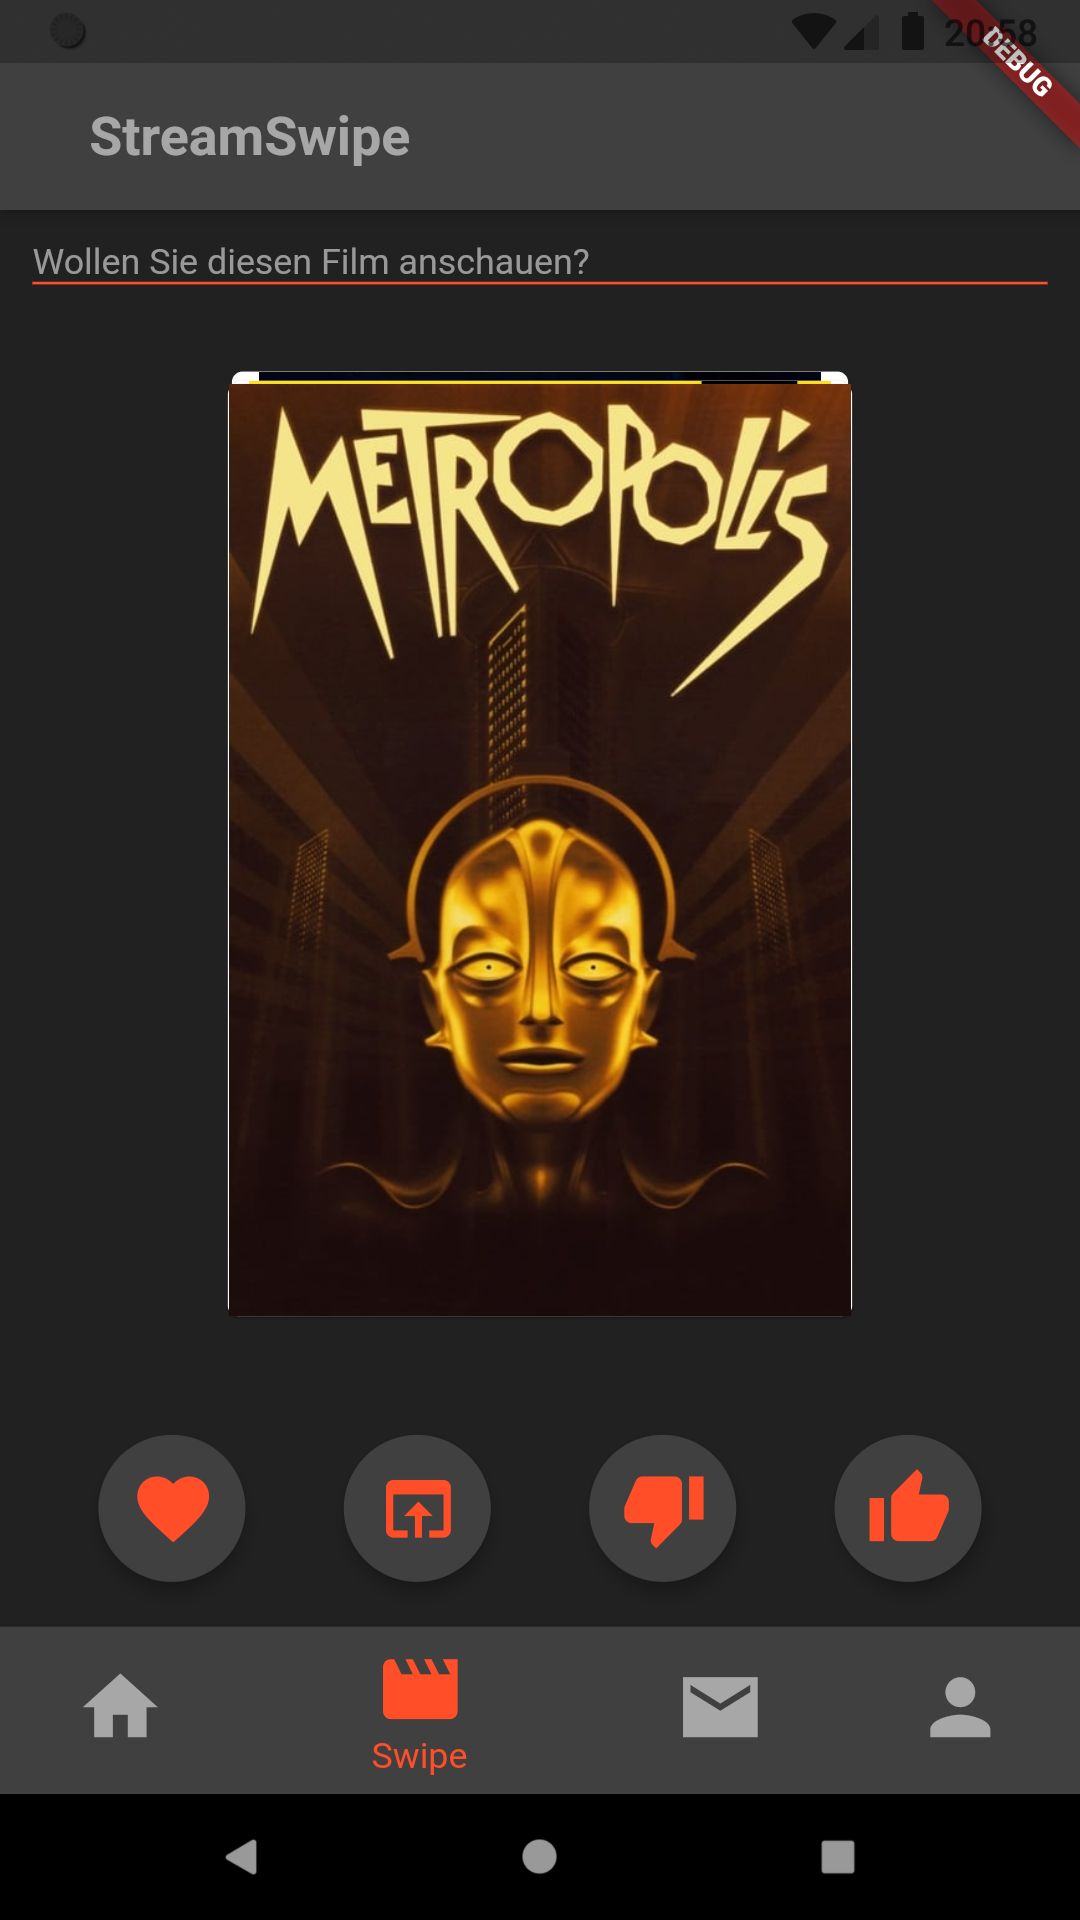
\includegraphics[scale=0.13]{Benutzeroberfläche/images/screenshot_darkmode_2.png}
	\caption{}
	\label{fig:swipescreen_e}
	\end{subfigure}
\caption[Screenshots der Swipe-Seiten]{Darstellungen und Funktionen der Swipe-Seiten mit (a) der Standarddarstellung, (b) weiteren Filminformationen, (c) einer Animation beim Drücken einer der Indikatoren und (d) der Swipe-Animation.  Hat der Nutzer in den Systemeinstellungen den dunklen Modus aktiviert, so wird (e) die Swipe-Seite wie alle anderen Seiten angepasst.}
\label{fig:swipescreen_alle}
\end{figure}
